\chapter{Pipeline Parallelism}

\section{Introduction}
\label{{sec:parallelism:pipeline_parallelism:intro}

	The basic idea of the data parallel is to distribute the model across GPUs. However, if the model size is bigger than the VRAM of GPU, the model wouldn't fit in a single GPU. To resolve the issue, we have to split the model across GPUs. For instance, we can put the half of the model into the fist GPU and the remaining half into the second GPU. This approach is often called \textit{model parallelism}. Let's closely look at one of the model parallelism approaches, called \textit{pipeline parallelism}. 

\textbf{Pipeline Parallelism is a strategy for distributing large deep learning models across multiple devices (GPUs) by splitting the model layers into sequential stages.} Rather than replicating the entire model on each GPU or sharding the parameters themselves, pipeline parallelism assigns a subset of layers to each device in a pipeline-like fashion. This technique is especially helpful when:
\begin{itemize}
	\item The model is too large to fit on a single GPU, but it can be split into chunks (layers/stages).  
	\item You want to keep multiple GPUs actively working on different portions (stages) of the forward and backward pass concurrently.
\end{itemize}


\subsection{Illustration of the Pipeline}

In pipeline parallelism, the model is divided into $N$ sub-networks, and each sub-network is placed on a different GPU (or sometimes on multiple GPUs if you have many layers). Think of it like an assembly line:
\begin{itemize}
	\item Sub-Network 1: Layers $1-k$  
	\item Sub-Network 2: Layers $(k+1)-m$ 
	\item Sub-Network 3: Layers$(m+1)-\dots$ 
	\item and so on.
\end{itemize}

The input minibatch is then split into smaller micro-batches (smaller pieces of data), which flow sequentially through these sub-networks. In other words, the micro-batch is the basic unit of the input to the pipeline parallelism. 
\begin{itemize}
	\item While Stage 1 is processing the next micro-batch, Stage 2 can concurrently work on the intermediate outputs from Stage 1's previous micro-batch.
\end{itemize}

\begin{figure}[t]
	\centering
	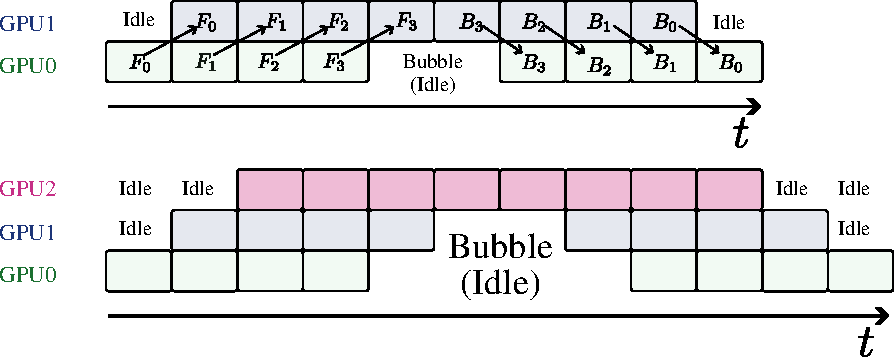
\includegraphics[scale=0.8]{./images/pipeline.pdf}
	\caption{The Illustration of the pipeline parallel on two GPUs. As you can see the \textit{bubble} (\ie underutilization) tends to grow as we increase the number of GPUs}
\end{figure}

\paragraph{Example:} Imagine a 2-stage pipeline parallel setup (for simplicity):

\begin{itemize}
	\item GPU 0: Holds Layers 1–3  
	\item GPU 1: Holds Layers 4–6  
\end{itemize}

If you have a batch of data with 32 samples, you might split it into 4 micro-batches of size 8 each. Then, forward Pass can be processed as follows:
\begin{enumerate}
	\item Micro-Batch 1
		\begin{enumerate}
			\item Step A: GPU 0 processes layers 1–3 for micro-batch #1.
			\item Step B: Once GPU 0 is done with those layers, it sends the activations for micro-batch #1 over to GPU 1.
			\item Step C: GPU 1 then processes layers 4–6 for micro-batch #1.
		\end{enumerate}
	\item Micro-Batch 2
		\begin{enumerate}
			\item As soon as GPU 0 finishes Step A for micro-batch #1 and passes the data to GPU 1, GPU 0 is free to start micro-batch #2 (layers 1–3).
			\item Meanwhile, GPU 1 is busy processing micro-batch #1 (layers 4–6).
			\item Once GPU 0 finishes its part for micro-batch #2, it sends those activations to GPU 1—which will be ready to handle them as soon as it’s done with micro-batch #1.
		\end{enumerate}
	\item Micro-Batch 3 and 4
		\begin{enumerate}
			\item This pattern continues in an overlapping fashion: while GPU 1 is busy with micro-batch #2, GPU 0 can start on micro-batch #3, and so on.
		\end{enumerate}
\end{enumerate}

The key benefit is concurrency:
\begin{itemize}
	\item While GPU 0 is processing micro-batch 2, GPU 1 can process micro-batch 1.  
	\item This overlap leads to higher GPU utilization.
\end{itemize}

Backward pass is a bit more complex because:
\begin{itemize}
	\item You need gradient signals to flow in the reverse order of the forward pipeline.  
	\item Each stage waits until it receives the gradient from the next stage before it can compute its own local gradients and pass them back to the previous stage.
\end{itemize}

However, the overall concept is similar-multiple stages can run backprop (on different micro-batches) in parallel, thereby keeping all GPUs busy.


\subsection{Pipeline Bubbles}

When using pipeline parallelism, you often hear about \textit{pipeline bubbles} (or underutilization). This refers to idle times on some GPUs before the assembly line is fully loaded or after it starts to wind down. 
\begin{itemize}
	\item Start-up Bubble: In the very beginning, GPU 1 must wait until GPU 0 finishes the first forward pass for micro-batch 1. GPU 1 sits idle during that initial delay.  
	\item Wind-down Bubble: After the last micro-batch enters GPU 0, GPU 1 continues to process the pipeline while GPU 0 is idle.
\end{itemize}

The percentage of idle can be computed as follows:
\begin{align*}
	\frac{1-m}{m+n-1},
\end{align*}
where $m$ is the number of microbatches and $n$ is the number of GPUs. 


These bubbles can lead to less-than-ideal speedups, but you can mitigate them by using enough micro-batches to keep the pipeline busy most of the time.

\subsection{Combining Pipeline Parallelism with Other Forms of Parallelism}

In practice, pipeline parallelism is often combined with:
\begin{itemize}
	\item Data Parallelism: You still replicate each stage across multiple GPUs to handle separate shards of data.  
	\item Tensor Parallelism / Model Parallelism: Instead of giving entire layers to one GPU, you split the parameters or compute of a single layer across multiple GPUs (common in large language model setups, \eg Megatron-LM).  
	\item Sharded Optimizer Approaches (\eg ZeRO, FSDP): Distribute optimizer states and gradients to reduce memory overhead.
\end{itemize}


\section{1F1B}

\begin{figure}[t]
	\centering
	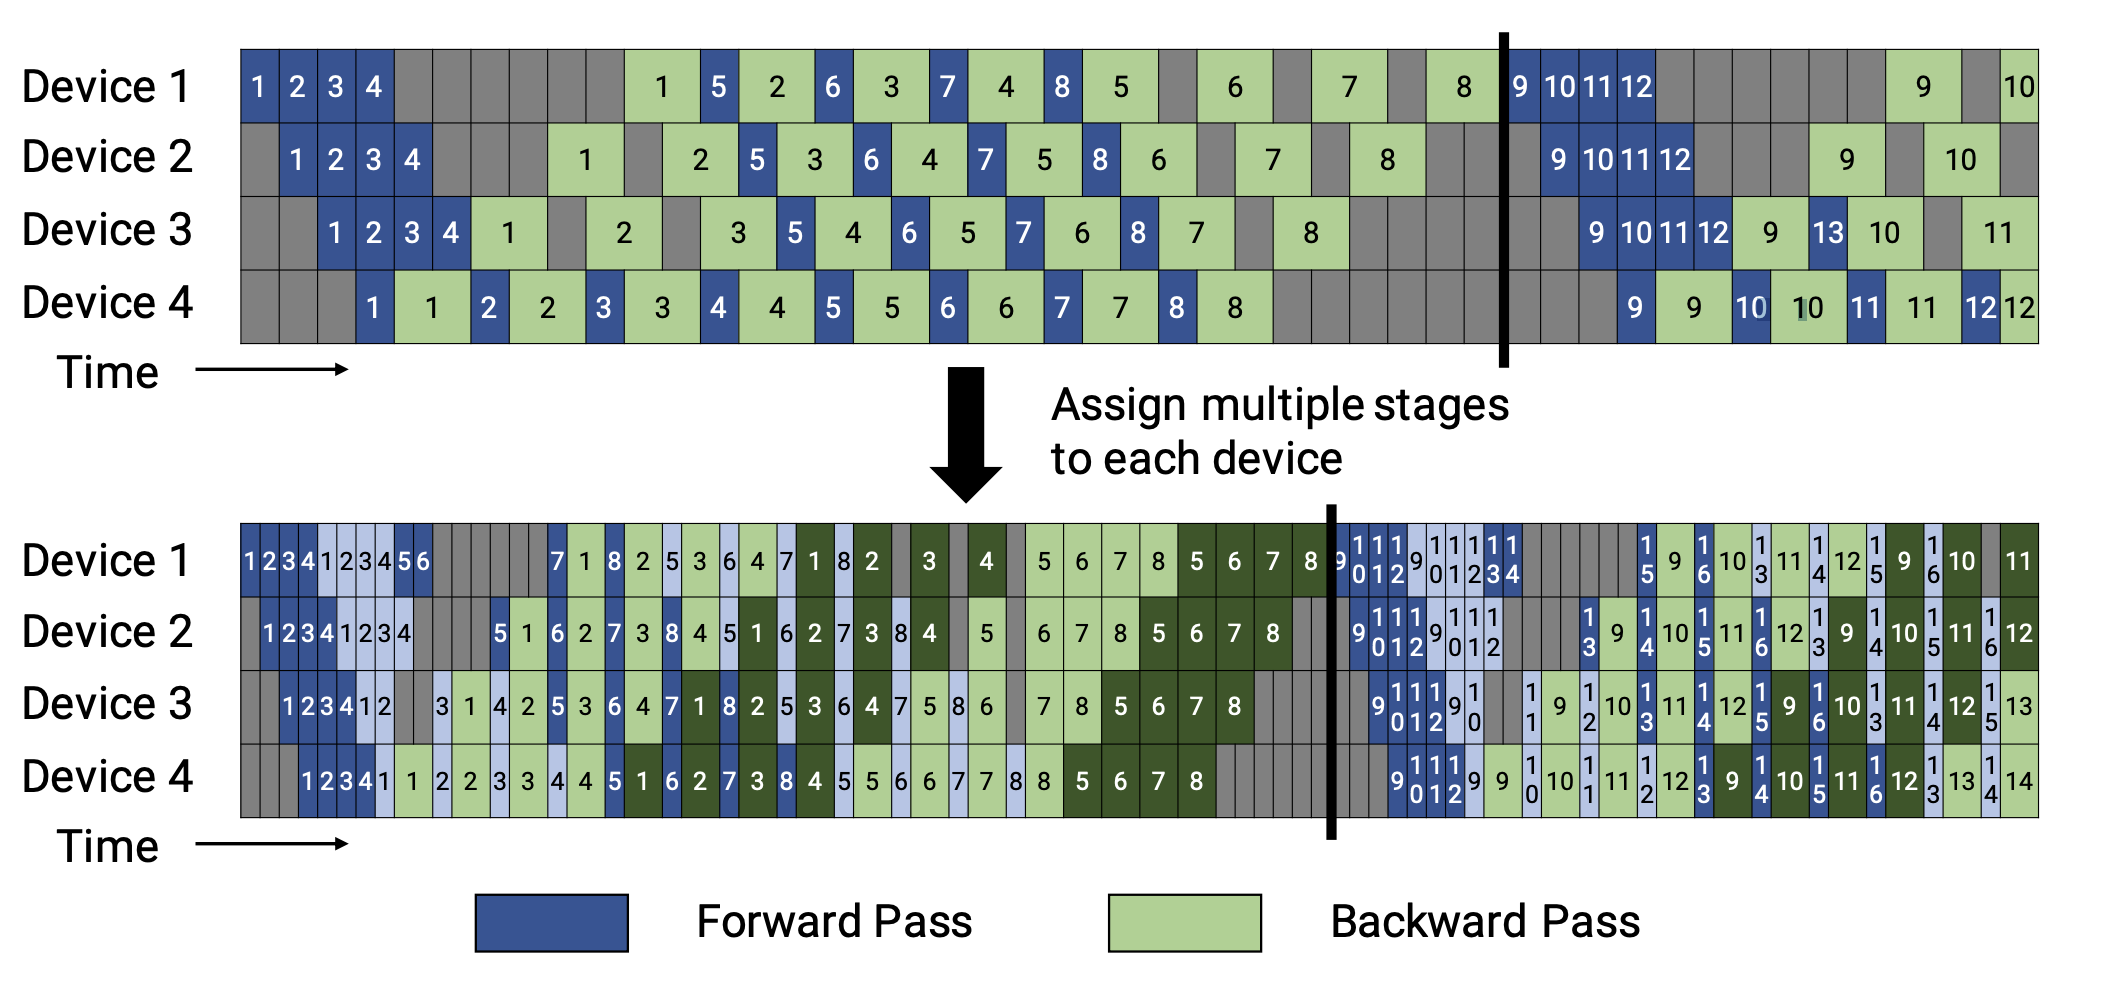
\includegraphics[scale=0.23]{./images/1f1b.png}
\end{figure}
One of the issues is that the model parameters keep changing while processing the forward passes. This means at every time step, minibatches are going to be forwarded through different weights. Thus, it is necessary to keep different states of the model parameters. Thus, 1F1B increases the memory requirements while increasing the processing speed. 

\subsection{Non-interleaved Schedule}

The non-interleaved schedule can be divided into two states. The first state is the startup state (or warm-up state). In the startup state, After completing the forward pass for the first minibatch, it performs the backward pass for the same minibatch, and then starts alternating between performing forward and backward passes for subsequent minibatches. As the backward pass starts propagating to earlier stages in the pipeline, every stage starts alternating between forward and backward pass for different minibatches. As shown in the above figure, in the steady state, every machine is busy either doing the forward pass or backward pass for a minibatch.

\subsection{Interleaved Schedule}

This schedule requires the number of microbatches to be an integer multiple of the stage of pipeline. In this schedule, each device can perform computation for multiple subsets of layers(called a model chunk) instead of a single contiguous set of layers. \ie Before device 1 had layer 1-4; device 2 had layer 5-8; and so on. But now device 1 has layer 1,2,9,10; device 2 has layer 3,4,11,12; and so on. With this scheme, each device in the pipeline is assigned multiple pipeline stages and each pipeline stage has less computation. This mode is both memory-efficient and time-efficient.



\section{Zero Bubble}
\label{sec:}
